\chapter{Device Concept}
The ultimate goal was to develop a system utilizing the FastIC+ chips that could be used at CERN to quickly carry out measurements, by companies to simplify prototyping with the FastIC+ chips, or by schools to use them in experiments. This implied the requirements for the system to be:
\begin{itemize}
    \item versatile to allow for both simple and demanding tasks,
    \item easy to use for both novices and experts,
    \item a standalone all-in-one device requiring no external scientific instruments,
    \item miniature and portable to be taken anywhere,
    \item financially available for schools and companies.
\end{itemize}

To allow for versatility, it was decided that two FastIC+ chips would be used, resulting in a total of 16 detection channels. The trigger inputs and outputs were decided to be exposed to the user to allow the synchronization of multiple readout boards. On the other hand, it was decided to read the data from the FastIC+ chips at the lowest possible speed of \SI{80}{\mega\bit\per\second}, as it was found sufficient for most applications and would greatly simplify the development.

To make the readout easy to use and standalone, a \emph{USB} interface was proposed to both power the device and transfer the data to a host computer for processing. This, in turn, required the device to be power-efficient and capable of sufficient \emph{USB} bandwidth.

Considering all of the above, it was decided to split the device into two parts: 
\begin{itemize}
    \item the readout board containing all the necessary electronics except the sensors,
    \item the easily replaceable user board containing mainly the sensors.
\end{itemize}

\chapter{Readout Board}
In the typical use case, a system integrating the FastIC+ chip would be based on an \emph{FPGA} with a dedicated \emph{Aurora} receiver or an \emph{FPGA} with a custom \emph{HDL} implementation of the receiver. This approach simplifies the implementation, as \emph{FPGAs} integrate the necessary deserializers and are capable of natively synchronizing to the data stream and reconstructing the data clock. However, the disadvantage is that sufficiently capable \emph{FPGAs} are expensive and power-hungry, which conflicts with the device's requirements. Another issue is that, while implementing an \emph{Aurora} receiver is relatively straightforward, implementing other interfaces like \emph{USB} is complex or requires purchasing expensive \emph{IP cores}. These drawbacks led to the decision to use a microcontroller for the readout system.

When a suitable microcontroller is selected, all the interfaces, such as:
\begin{itemize}
    \item \emph{ADCs} for monitoring voltages,
    \item \emph{DACs} for providing voltage feedback,
    \item \emph{SPI} and \emph{I2C} for communication with other digital devices,
    \item \emph{USB} for connection to the host,
\end{itemize}
are implemented in hardware and do not need to be defined in \textit{HDL}. A simple firmware in C/C++ can then be developed to control these interfaces, potentially speeding up and simplifying development while allowing more users to easily customize the device's functionality. The main challenge with this approach is that no microcontroller on the market implements the receivers or deserializers required to recover the clock from the \emph{Aurora} stream and synchronize to it. Therefore, clock recovery must be performed externally, and a suitable alternative peripheral must be chosen to serve as the receiver.

\section{Microcontroller}
The STM32H753XIH6 was chosen as an excellent microcontroller candidate for the system. It is based on an Arm Cortex-M7 core running at up to \SI{480}{\mega\hertz}, which provides the fast computation required for processing the two continuous \SI{80}{\mega\bit\per\second} streams. It integrates \SI{2}{\mega\byte} of flash memory and \SI{1}{\mega\byte} of RAM, which is more than sufficient for buffering the data. From a peripheral perspective, it supports \emph{USB High Speed} with a maximum throughput of \SI{480}{\mega\bit\per\second}, which is essential for transferring the large amount of data to the host. It also features multiple \emph{SPI} peripherals supporting input clocks of up to \SI{120}{\mega\hertz}, making them an ideal choice for sampling the \emph{Aurora} stream running at \SI{80}{\mega\bit\per\second}, as explained in \ref{sec:aurora_sampling}. The internal data buses of the microcontroller operate at half the core clock speed and support \emph{DMA}, which significantly enhances performance when handling such a large amount of data. In addition to these main features, the chip's implementation of two \emph{ADCs}, one \emph{DAC}, and \emph{I2C} for digital communication is also beneficial for the readout. The chip is packaged in a compact \SI{14}{\milli\meter} $\times$ \SI{14}{\milli\meter} \emph{TFBGA} 240+25 package.

\subsection{Receiving the Aurora stream}
\label{sec:aurora_sampling}
As noted above, the most suitable peripheral for receiving the \emph{Aurora} stream with this microcontroller is the \emph{SPI} peripheral. This peripheral is an industry-standard serial interface, implemented in all modern \textit{MCUs}, designed for receiving a serial stream with a dedicated clock. In simplex slave, receiver-only mode, which suits this use case well, the peripheral uses the \verb|CLK| and \verb|MOSI| pins. The \verb|MOSI| pin is used to input the data stream into the peripheral. The clock, present on the \verb|CLK| pin, is then used to sample the data stream. The sampled data is shifted into a register on a selected clock edge and sent over the internal microcontroller buses for processing. The only challenge with using \emph{SPI} is that the need to recover the clock from the data stream remains.

\subsection{Omitting clock recovery with the FastIC+}
As noted in Section \ref{sec:fastic}, the FastIC+ requires a \SI{40}{\mega\hertz} reference clock to function. The chip features an internal \emph{PLL}, which synchronizes to this clock and distributes it to other peripherals, including the \emph{Aurora} transmitter. Since the \emph{PLL} phase is phase-locked to the input clock, the \emph{Aurora} transmitter, and thus the \emph{Aurora} output stream, is also phase-locked to the input clock, just delayed by the transmitter propagation delay $t_{pd}$. Measurements have shown that this delay is very stable across a temperature range of \SI{0}{\celsius} to \SI{100}{\celsius}, with a value of $t_{pd}$ = \SI{3.48 (0.08)}{\nano\second}. If this delay is combined with an additional controlled delay, the digital stream can be aligned such that the data can be sampled with an \SI{80}{\mega\hertz} sampling clock that is in phase with the FastIC+ reference clock.

The delay could be implemented using a variable delay line. However, the $t_{pd}$ of the FastIC+, combined with the typical propagation delay of a common \emph{LVDS-to-CMOS} receiver (typically \SI{5}{\nano\second}), equals approximately \SI{9}{\nano\second}. The \emph{Aurora} data stream operates at double data rate, meaning a valid symbol is transferred on both the rising and falling edges of the reference clock. This results in a symbol duration of \SI{12.5}{\nano\second}. The \SI{9}{\nano\second} delay, being almost exactly $3/4$ of the symbol duration, shifts the data so that both sampling clock edges fall within the data symbol, as shown in Figure \ref{fig:clock_align}. Consequently, the data symbol can be sampled on either the rising or falling edge, and the edge can be selected programmatically based on the receiver propagation delay to avoid sampling in a metastable state. Since the FastIC+ outputs an \emph{SLVS} signal and an \emph{MCU} with \emph{CMOS} inputs is used to capture the stream, this receiver must be present anyway. If carefully chosen, it can also serve as the delay line to achieve the correct sampling clock phase, thereby completely eliminating the need to recover the clock from the data stream.
\FloatBarrier
\begin{figure}[htp!]
    \centering
    \begin{tikztimingtable}[%
        timing/dslope=0.1,
        timing/.style={x=5ex,y=2ex},
        x=5ex,
        timing/rowdist=3ex,
        %timing/name/.style={font=\sffamily\scriptsize}
    ]
    Reference Clock        & u 2{hhhhllll} hhhh \\
    Sampling Clock         & un(A1) 5{hhll} \\
    Data                   & uuuun(A2) 4d{} 4d{} 4d{} 4d{} d\\
    \extracode
    \begin{pgfonlayer}{background}
    \begin{scope}[semitransparent ,semithick]
        \vertlines[darkgray,dotted]{0.5,1,1.5 ,...,8.0}
    \end{scope}
    \end{pgfonlayer}

    \draw [<->] ([shift=({0,-3})]A1|-row2.mid) --node[below]{\scriptsize{$\approx$ \SI{9}{\nano\second}}} ([shift=({0,-3})]A2|-row2.mid);


    \end{tikztimingtable}
    \caption{Alignment of the sampling clock and data stream}
    \label{fig:clock_align} 
\end{figure}
\FloatBarrier
\section{FastIC+}
As mentioned above, the FastIC+ requires almost no additional components aside from a \SI{1.2}{\volt} power source and the \SI{40}{\mega\hertz} reference clock. The XVDD (\emph{PLL}) power domain has been isolated from the TVDD (threshold circuitry) by a ferrite bead to reduce noise coupling between the two. However, the \emph{PLL} is only expected to produce noise at startup, while the threshold circuitry is used only after the \emph{PLL} has locked, so any noise coupling between the two domains should have little to no impact. All of the power domains have been thoroughly decoupled, as seen in Figure \ref{fig:fastic_power}.
%
\FloatBarrier
\begin{figure}[htp!]
    \centering
    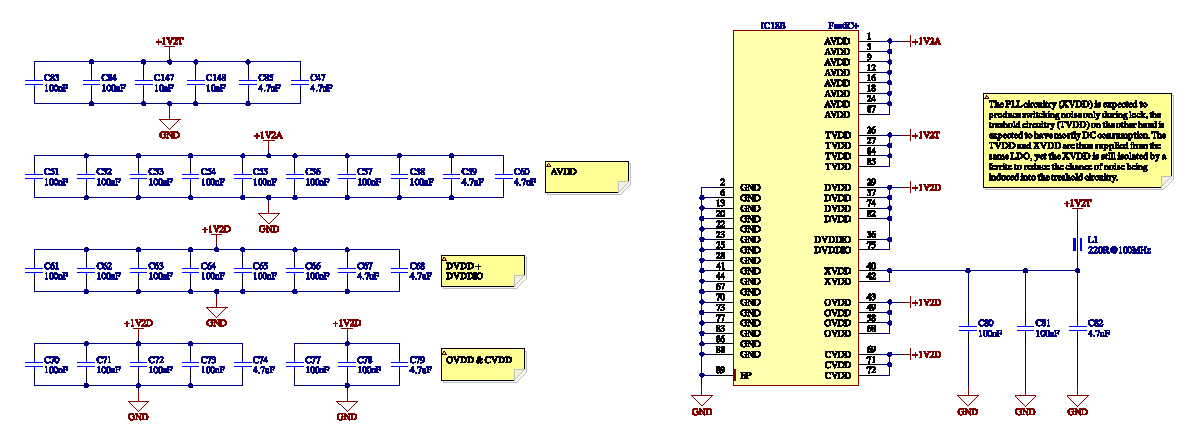
\includegraphics[scale=0.6]{schematic/fastic_power.eps}
    \caption{Schematic of the FastIC+ power}
    \label{fig:fastic_power}
\end{figure}
\FloatBarrier
%
To increase the stability of the internal bandgap reference, a \SI{10}{\nano\farad} capacitor has been added to the \verb|VBG| pin according to the datasheet.

Both \verb|nRST| (reset of the FastIC+) and \verb|SRST| (reset of the synchronous counter) have been pulled up to the digital supply so that the microcontroller pins in open drain mode can be used to control these without the need for voltage translation. 

\FloatBarrier
\begin{figure}[htp!]
    \centering
    \includegraphics[scale=0.6]{schematic/fastic.eps}
    \caption{Schematic of the FastIC+ logic}
    \label{fig:fastic}
\end{figure}
\FloatBarrier


%
\subsection{I2C communication}
As the FastIC+ voltage domains all run at \SI{1.2}{\volt}, a voltage shifter had to be implemented for communication with the microcontroller over \emph{I2C}. For this, the PCA9306DQER has been chosen for its miniature \emph{X2SON} package and sufficent \SI{400}{\kilo\hertz} speed. 
%
\subsection{Calibration pulse generator}
The FastIC+ features a \verb|CAL| input pin used for injecting a test pulse into any of the eight input channels. This pin converts the pulse to current with an internal \SI{70}{\ohm} resistor. The usual shape of such a pulse should resemble a real sensor output, thus a decaying exponential with an amplitude of a few milliamperes and a length under a microsecond. To create this pulse, a high-side switch has been implemented with series resistance to limit the current and parallel capacitance to recreate the decaying exponential. The transistor gate is driven by a quick digital pulse from the microcontroller, whose length can be adjusted to modify the current pulse width and, to some degree, also the amplitude.
%
\subsection{Voltage monitoring}
%
The \verb|VMON| pin on the ASIC serves for monitoring the internal analog thresholds and \emph{DAC} outputs. Since the microcontroller's internal voltage reference has been selected to run at \SI{1.8}{\volt}, a simple non-inverting amplifier with a voltage gain of
%
\begin{equation}
    A_V = \left( 1 + \frac{R41}{R44}\right) = \left( 1 + \frac{\SI{10}{\kilo\ohm}}{\SI{20}{\kilo\ohm}}\right) = 1.5
\end{equation}
%
has been implemented to amplify the \SI{1.2}{\volt} output to the microcontroller's full-scale range and improve performance. Because the \verb|VMON| output is used only for threshold monitoring, thus only DC voltages, a slow RC filter has been used to reduce the noise coupled to the analog signal.
%
\FloatBarrier
\begin{figure}[htp!]
    \centering
    \includegraphics[scale=2]{schematic/fastic_vmon.eps}
    \caption{Schematic of the voltage monitoring amplifier}
    \label{fig:fastic_vmon}
\end{figure}
\FloatBarrier
%
\subsection{High speed outputs}
%
The FastIC+ outputs use the \emph{Scalable Low Voltage Signaling} standard. \emph{SLVS} is an alternative to \emph{LVDS}, utilizing lower voltages. The transmitter common mode voltage $V_{CMTX}$ is \SI{0.6}{\volt}, and the differential voltage $|V_{OD}|$ is \SI{0.2}{\volt}, as shown in Figure \ref{fig:slvs_voltages}.

\begin{figure}[ht]
	\begin{center}
		\includegraphics[scale=0.8]{06_SLVS_specs.pdf}
	\end{center}
	\vspace{-5mm}
	\caption{Voltage definition for SLVS transmitter}
	\label{fig:slvs_voltages}
\end{figure}

A differential output capable of transmitting a pulse whose beginning timestamps the \emph{ToA} of a photon and whose length resembles the \emph{ToT} is present on the FastIC+ for each channel separately. However, as the readout uses the data digitized by the internal \emph{TDC}, these channels are left unconnected and disabled in the chip to reduce \emph{EMI}.

The \verb|TIME| output can be internally connected to the trigger comparator and used for the trigger threshold calibration routine. That's why it was also interfaced with the microcontroller. When the pin is not used for calibration, it is disabled to reduce any \emph{EMI} generated by the fast edges. The \verb|TDCOUT| is the output of the \emph{Aurora} stream from the transmitter.

Both of the above-mentioned pins are connected to the DS90LVRA2 dual-channel differential line receiver and terminated by a \SI{100}{\ohm} resistance, corresponding to the impedance of the differential lines. This receiver, used to convert the \emph{SLVS} output to \emph{CMOS}, has been chosen specifically for its small size, high enough speed, and typical propagation delay $t_{pd}$ = \SI{4.4}{\nano\second} to correctly align the data to the sampling clock. Even though it is intended to convert \emph{LVDS} signals, the threshold voltage levels work well with the \emph{SLVS} standard mentioned above, thus no other special circuitry is needed. 

\subsection{Trigger input and output}
The trigger inputs (used for externally triggering the ASIC) and outputs (outputting the signal from the internal comparator) have been exposed to the user on two \emph{SMA} connectors. Termination has been placed on these to mitigate any reflections, and \emph{ESD} protection diodes have been added to protect the chip from electrostatic discharge. It's important to note that the \emph{ESD} diodes add capacitance to the trigger lines, thus degrading (slowing) the trigger edge and introducing a slight delay in the trigger. This either needs to be accounted for when using the readout, or the diodes need to be left unassembled at the expense of worse \emph{ESD} immunity. 
%
\FloatBarrier
\begin{figure}[htp!]
    \centering
    \includegraphics[scale=1.6]{schematic/fastic_top.eps}
    \caption{Schematic of the FastIC+ trigger circuitry}
    \label{fig:schem_fastic_triggers}
\end{figure}
\FloatBarrier

\section{USB}
To supply power to the device and handle communication with the host computer, a \emph{USB Type-C} connector has been used.
\FloatBarrier
\begin{figure}[htp!]
    \centering
    \includegraphics[scale=.75]{schematic/usb_con.eps}
    \caption{Schematic of the USB connector with ESD protection}
    \label{fig:schem_usb_con}
\end{figure}
\FloatBarrier
\subsubsection{External PHY}
Because the combined data rate of the FastIC+ chips of \SI{160}{\mega\bit\per\second} exceeds the \emph{USB 1.1} specification, \emph{USB 2.0} (High Speed) was implemented, supporting up to \SI{480}{\mega\bit\per\second} throughput. Unfortunately, the microcontroller used does not integrate the \emph{USB 2.0 PHY} directly. Instead, it only integrates the necessary logic and interfaces with an external \emph{PHY} via the \emph{ULPI} interface. 

A USB3320 interface was chosen as it is well-supported by the microcontroller and widely used in countless designs. A \SI{48}{\mega\hertz} crystal oscillator has been used as the external reference clock required for the device to operate. Different crystal frequency selections have been made possible with \SI{0}{\ohm} resistor jumpers. The \emph{ULPI} connections have been series-terminated to better match the driver output impedance to the controlled impedance of the line.
\FloatBarrier
\begin{figure}[htp!]
    \centering
    \includegraphics[scale=.68]{schematic/usb.eps}
    \caption{Schematic of the USB}
    \label{fig:schem_usb}
\end{figure}
\FloatBarrier
\subsubsection{Power Delivery}
A FUSB302 chip was added to allow for power limit negotiation with a \emph{UCPD} capable power source. The chip handles all the necessary signaling and communicates with the \emph{MCU} via a \emph{I2C} interface. Optional \SI{5.1}{\kilo\ohm} resistors have been added to passively negotiate the highest power limit, if it would be decided to omit the power delivery functionality and not assemble the FUSB302.
\FloatBarrier
\begin{figure}[htp!]
    \centering
    \includegraphics[scale=.9]{schematic/ucpd.eps}
    \caption{Schematic of the UCPD controller}
    \label{fig:schem_ucpd}
\end{figure}
\FloatBarrier
\subsection{Clock generation}
To generate the \SI{40}{\mega\hertz} reference clock for both of the FastIC+ chips and the \SI{80}{\mega\hertz} sampling clock for the \emph{SPI} peripherals, the SI5340 clock synthesizer has been used. It features four outputs with \SI{90}{\femto\second} \emph{RMS} jitter, supporting both \emph{CMOS} and differential output. Additionally, each output can be powered by an independent power supply, allowing for mixing the \SI{3.3}{\volt} \emph{CMOS} signals for the microcontroller and differential signals for the FastIC+. A precise \SI{48}{\mega\hertz} crystal oscillator has been used as the reference clock. The chip features both \emph{I2C} and \emph{SPI} interfaces for configuration. \emph{I2C} was selected for use in this design.

\FloatBarrier
\begin{figure}[htp!]
    \centering
    \includegraphics[scale=0.65]{schematic/clock.eps}
    \caption{Schematic of the clock generator}
    \label{fig:schem_clock}
\end{figure}
\FloatBarrier

Since the FastIC+ requires an \emph{SLVS} input, which is not supported by the generator, a signal divider had to be implemented. This circuit, shown in Figure \ref{fig:schem_slvs}, was provided in the datasheet to lower the voltage levels while keeping the impedance of the lines well-matched.
\FloatBarrier
\begin{figure}[htp!]
    \centering
    \includegraphics[scale=2]{schematic/slvs.eps}
    \caption{Divider for the LVDS to SLVS conversion}
    \label{fig:schem_slvs}
\end{figure}
\FloatBarrier

\subsection{High Voltage}
All the sensors that the FastIC+ interfaces with, such as \emph{SiPMs}, \emph{PMTs}, or \emph{MCPs}, require high-voltage biasing for their operation. To eliminate the need for an external high-voltage supply, an internal one has been implemented using the LT3571. This DC/DC converter, designed for biasing avalanche photodiodes, is capable of generating up to \SI{75}{\volt} output from a low-voltage input. It fully integrates the power switch and regulation along with soft-start and variable switching frequency. This has been set to approximately \SI{1}{\mega\hertz} via \verb|R61|. A higher switching frequency allowed for the use of smaller inductance, thereby keeping the size of the device compact.

\FloatBarrier
\begin{figure}[htp!]
    \centering
    \includegraphics[scale=.65]{schematic/hv.eps}
    \caption{High voltage power supply schematic}
    \label{fig:schem_hv}
\end{figure}
\FloatBarrier
A \verb|CTRL| input is available for adjusting the output with a control voltage. This reference is generated by the \emph{MCU} \emph{DAC} and divided by a voltage divider to a suitable \SI{0}{V} - \SI{1}{V} range. The feedback resistor divider was chosen such that the theoretical maximum output voltage, with the \verb|CTRL| pin held at \SI{1}{\volt}, is \SI{84.3}{\volt}, as shown in equation \ref{eq:hv_voltage_fb}.

\begin{equation}
V_{MONIN} = (\frac{R57}{R62} + 1) \cdot V_{CTRL} = (\frac{\SI{1000}{\kilo\ohm}}{\SI{12}{\kilo\ohm}} + 1) \cdot \SI{1}{\volt} = \SI{84.3}{\volt}
\label{eq:hv_voltage_fb}
\end{equation}


The current limit resistor has been chosen to limit the \verb|APD| pin current to approximately \SI{8}{\milli\ampere} based on the equation \ref{eq:hv_current_limit} mentioned in the datasheet.

\begin{equation}
R_{SENSE} = \frac{\SI{200}{\milli\volt}}{1.2 \cdot I_{APD} + \SI{0.3}{\milli\ampere}} \approx \SI{20}{\ohm}
\label{eq:hv_current_limit}
\end{equation}
%
where $I_{APD}$ is the \verb|APD| pin current limit in milliamperes.
To allow for closed-loop control with the microcontroller, the output voltage on the \verb|APD| pin is monitored via a suitable voltage divider with an operational amplifier buffer. For current monitoring, the LT3571 offers the \verb|IMON| pin, which sources a current $I_{IMON} = 0.2 \cdot I_{APD}$. This current is then converted to voltage with a \SI{1}{\kilo\ohm} resistor and buffered with an operational amplifier.

\FloatBarrier
\begin{figure}[htp!]
    \centering
    \includegraphics[scale=.8]{schematic/hv_isense.eps}
    \includegraphics[scale=.8]{schematic/hv_usense.eps}
    \caption{Sensing of the high voltage and current}
    \label{fig:schem_hvsense}
\end{figure}
\FloatBarrier

\subsection{Power}
A DC/DC converter has been implemented to efficiently lower the \SI{5}{\volt} input voltage to the \SI{3.3}{\volt} used by the microcontroller. The \SI{3.3}{\volt} for the analog domain has been generated with a low ripple \emph{LDO}. The \SI{1.8}{\volt} domain for the \emph{USB} interface has been derived from the \SI{3.3}{\volt} using an \emph{LDO} aswell, as efficiency is not required with the low power consumption of \SI{29.4}{\milli\ampere} of the \SI{1.8}{\volt} domain.
\FloatBarrier
\begin{figure}[htp!]
    \centering
    \includegraphics[scale=1]{schematic/power_dcdc.eps}
    \caption{Step down regulator schematic}
    \label{fig:schem_dcdc}
\end{figure}
\FloatBarrier

Power sequencing has been implemented for all the three FastIC+ voltage domains. First, the digital domain supply is activated, followed by the supply for the treshold circuitry and \emph{PLL} and lastly, the analog domain is supplied. All of these domains are derived from the \SI{3.3}{\volt} using a \SI{1.2}{\volt} \emph{LDOs} which are sufficient for the low power consumption (\SI{113}{\milli\ampere} per chip) and provide a ripple-free supply for the sensitive treshold circuitry.

\FloatBarrier
\begin{figure}[htp!]
    \centering
    \includegraphics[scale=.55]{schematic/power_fastic.eps}
    \caption{FastIC+ power domain sequencing}
    \label{fig:schem_fastic_power}
\end{figure}
\FloatBarrier

\section{Connector}
To interface with the user board, the \SI{9}{\milli\meter} high version of the ERM8-020 connector has been used due to its durability (up to 1000 connection cycles), good high-speed performance, and suitable pin count. This connector carries all sixteen input channels alongside the high-voltage biasing supply. The \SI{3.3}{\volt} supply is also exposed, and four pins are dedicated to user board identification.
%
\subsubsection{Identification pins}
The identification pins serve as an easy way to assign a four-bit short ID to a specific user board. This ID can then be used by the software to load a configuration preset defined for the user board. If the user board designer decides to, the pins \verb|ID0| and \verb|ID1| can be used as \emph{I2C} communication lines. A compatible \emph{EEPROM} can then be assembled on the user board, making it possible to save the full configuration on the user board itself, as well as additional data such as the name or a unique ID. If the \emph{I2C} interface is to be used, all of the ID pins need to be pulled up high by a suitable resistor. At least one of the ID pins has to be high at all times. This means that an ID of \verb|0b0000| is not allowed, and in this case, the readout will not recognize a valid user board. 
%
\chapter{User board}
The user board has been developed as a template for users to easily get started with the readout system. It contains a matrix of 4 $\times$ 4 \emph{SiPM} sensors as well as an \emph{EEPROM} for storing the board configuration. The \SI{9}{\milli\meter} high ERF8-020 connector has been chosen for the user board to match the counterpart present on the readout and allow enough clearance between the assembled readout board and user board.

\section{Sensors}
The footprint for generic THT \emph{SiPMs} has been implemented on the board. Each \emph{SiPM} is biased with the high voltage, and the input is filtered with a dual RC low pass to eliminate the possibility of cross-triggering of the sensors. 

\FloatBarrier
\begin{figure}[htp!]
    \centering
    \includegraphics[scale=1.2]{schematic/sipm.eps}
    \label{fig:sipm}
\end{figure}
\FloatBarrier

\section{EEPROM}
The 24AA04T-I/OT \SI{4}{\kilo\bit} \emph{EEPROM} has been used on the user board for the configuration storage. It has been selected for the low price and sufficient capacity. 

\newpage
\chapter{PCB design}
Special care had to be taken when designing the PCB, keeping in mind the correct design practices for propper power integrity, signal integrity and high speed design. 

First a suitable stackup was chosen. In this case, it was decided to proceed with an eight layer stackup as shown in table \ref{tab:stackup}. 
\FloatBarrier
\begin{table}[htp!]
    \caption{PCB stackup}
    \begin{tabular}{|l|l|l|}
    \hline
    \multicolumn{1}{|c|}{\textbf{Layer}} & \multicolumn{1}{c|}{\textbf{Name}} & \multicolumn{1}{c|}{\textbf{Thickness}} \\ \hline
    1                                    & L1 - Top copper                    & \SI{0.018}{\milli\meter}                                   \\ \hline
                                         & Dielectric - PR2116                & \SI{0.120}{\milli\meter}                                   \\ \hline
    2                                    & L2 - Ground plane                  & \SI{0.035}{\milli\meter}                                   \\ \hline
                                         & Dielectric - FR4 core              & \SI{0.200}{\milli\meter}                                   \\ \hline
    3                                    & L3 - Power plane                   & \SI{0.035}{\milli\meter}                                   \\ \hline
                                         & Dielectric - PR2116                & \SI{0.120}{\milli\meter}                                   \\ \hline
                                         & Dielectric - PR2116                & \SI{0.120}{\milli\meter}                                   \\ \hline
    4                                    & L4 - Signal layer                  & \SI{0.035}{\milli\meter}                                   \\ \hline
                                         & Dielectric - FR4 core              & \SI{0.200}{\milli\meter}                                   \\ \hline
    5                                    & L5 - Signal layer                  & \SI{0.035}{\milli\meter}                                   \\ \hline
                                         & Dielectric - PR2116                & \SI{0.120}{\milli\meter}                                   \\ \hline
                                         & Dielectric - PR2116                & \SI{0.120}{\milli\meter}                                   \\ \hline
    6                                    & L6 - Power plane                   & \SI{0.035}{\milli\meter}                                   \\ \hline
                                         & Dielectric - FR4 core              & \SI{0.200}{\milli\meter}                                   \\ \hline
    7                                    & L7 - Ground plane                  & \SI{0.035}{\milli\meter}                                   \\ \hline
                                         & Dielectric - PR2116                & \SI{0.120}{\milli\meter}                                   \\ \hline
    8                                    & L8 - Bottom copper                 & \SI{0.018}{\milli\meter}                                   \\ \hline
    \end{tabular}
    \label{tab:stackup}
\end{table}
\FloatBarrier
The layers 2 and 3, as well as layers 6 and 7, were completely dedicated to ground and power planes. This, in combination with relatively thin dielectric in between, creates inherent capacitive coupling between the planes proportional to the plane area and spacing, which helps the power integrity of the device. %For a board of size $\SI{50}{\milli\meter} \times \SI{50}{\milli\meter}$, which is the case for the readout, and the stackup mentioned, this capacitance can be estimated using the equation for a parallel plate capacitor to be
%
%\begin{equation}
%C = \varepsilon_0 \cdot \varepsilon_r \cdot \frac{S}{d} = \SI{8.85e-12}{\farad\per\meter} \cdot 4.2 \cdot \frac{\SI{2500}{\milli\meter\squared}}{\SI{0.2}{\milli\meter}} = \SI{465}{\pico\farad}
%\end{equation}
%
Leaving the planes solid also keeps the impedance minimal which reduces the voltage drops. The layers 4 and 5 were also mostly kept as planes, although some connections needed to be routed through these because of the very high board density. While routing in these layers, care was taken not to cross possible return current paths of the planes with another trace, which could result in a much bigger current loop and an increase in \emph{EMI}. Layers 1 and 8, the top and bottom copper, were used mainly for routing of all the signals. Since both of the layers have a ground plane underneath, both of them were used for routing of the high speed lines with defined impedance. 
%
\section{High speed signals}
To mitigate possible reflections on the high-speed lines carrying high-frequency signals, the characteristic impedance of each line was calculated to match the driver impedance. For differential signals, the differential impedance was optimized to be \SI{100}{\ohm}, except for the USB lines, which require a differential impedance of \SI{90}{\ohm}. For single-ended lines, the target impedance was \SI{50}{\ohm}.
The line widths, as well as the spacing for differential pairs, were calculated using Altium Designer’s impedance calculator and verified using the PCB manufacturer’s impedance calculation tool. These calculations resulted in a width of $W_{USB} = \SI{0.183}{\milli\meter}$ and spacing of $S_{USB} = \SI{0.2}{\milli\meter}$ for the USB differential pair; a width of $W_{DIFF} = \SI{0.15}{\milli\meter}$ and spacing of $S_{DIFF} = \SI{0.2}{\milli\meter}$ for the remaining differential pairs; and a width of $W_{SE} = \SI{0.182}{\milli\meter}$ for all single-ended high-speed lines. The spacing from the ground plane on these was kept as large as possible to avoid affecting the impedance. These widths and spacings were followed during PCB routing to ensure the trace impedances remained as close to their respective targets as possible. Where necessary, the line lengths and skews were matched. Routing of the \emph{ULPI} interface and FastIC+ clock lines can be seen in Figure \ref{fig:highspeed}.

\FloatBarrier
\begin{figure}[htp!]
    \centering
    
\includegraphics[height=8cm]{high_speed.eps}
    \caption{High speed signal lines}
    \label{fig:highspeed}
\end{figure}
\FloatBarrier

\section{Microcontroller fanout}
Care was taken to properly fan out the microcontroller pins to avoid any signal integrity issues. First, the pinout was optimized to place the high-speed lines along the perimeter of the package, allowing them to be routed as directly as possible. Decoupling capacitors were then placed on the bottom side of the PCB, as close to the power pins as possible, in order to minimize connection inductance and current loop area. The remaining low-speed connections were routed in the leftover space. Routing under the microcontroller can be seeen in Figure \ref{fig:fanout}.

\FloatBarrier
\begin{figure}[htp!]
    \centering
    
\includegraphics[height=8cm]{fanout.eps}
    \caption{Microcontroller fanout}
    \label{fig:fanout}
\end{figure}
\FloatBarrier

\section{Power integrity}
The power integrity of the device was ensured by using solid power and ground planes, as previously described. Capacitors were placed as close as possible to the power pins of the decoupled integrated circuits and connected to the planes using vias, in order to minimize the inductance of the current loops. The ground planes were stitched together with via array. Additional care was taken to place ground vias near locations where high-speed lines transition between the top and bottom \emph{PCB} layers. Since the current of a high-speed signal in a transmission line is concentrated in close proximity to the signal trace, the corresponding return current flows along the adjacent ground plane. By placing ground vias next to the signal vias, the return path is preserved, minimizing the loop area and reducing emitted \emph{EMI}.

\section{Design files}
Gerber files were generated using Altium Designer and were made available on the \emph{GitHub} repository. The PCB was designed to be as compact as possible, with a size of \SI{50}{\milli\meter} $\times$ \SI{50}{\milli\meter}. Top and bottom layers can be seen bellow.

\FloatBarrier
\begin{figure}[htp!]
    \centering
    
\includegraphics[height=8cm]{top_layers.eps}
    \caption{Top metal layer}
    \label{fig:metal_top}
\end{figure}
\FloatBarrier

\FloatBarrier
\begin{figure}[htp!]
    \centering
    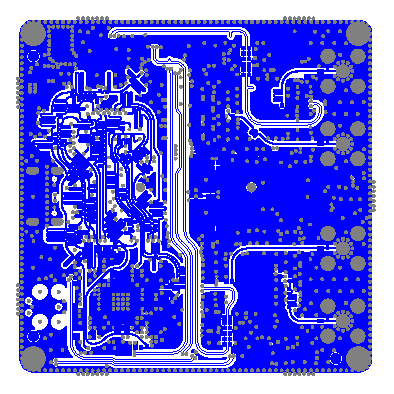
\includegraphics[height=8cm]{bot_layers.eps}
    \caption{Bottom metal layer}
    \label{fig:metal_bot}
\end{figure}
\FloatBarrier

\section{Manufacturing}
The two PCBs described above were manufactured and assembled by Eurocircuits. The 3D renders as well as actual photos of the assembled PCBs can be seen in the images bellow. 



\FloatBarrier
\begin{figure}[htp!]
    \centering
    \includegraphics[height=5.2cm]{readout_3d-top.png}
    \includegraphics[height=5.2cm]{readout_3d-bottom.png}
    \caption{Readout PCB}
    \label{fig:readout_3d}
\end{figure}
\FloatBarrier

\FloatBarrier
\begin{figure}[htp!]
    \centering
    \includegraphics[height=5.2cm]{userboard_3d-top.png}
    \hspace{1.8cm}
    \includegraphics[height=5.2cm]{userboard_3d-bottom.png}
    \caption{User board PCB}
    \label{fig:userboard_3d}
\end{figure}
\FloatBarrier


\FloatBarrier
\begin{figure}[htp!]
    \centering
    \includegraphics[height=5.3cm]{photo_readout_top.png}
    \includegraphics[height=5.3cm]{photo_readout_bot.png}
    \caption{Manufactured readout PCB}
    \label{fig:photos_readout}
\end{figure}
\FloatBarrier

\FloatBarrier
\begin{figure}[htp!]
    \centering
    \includegraphics[height=5.55cm,trim={2cm 0 0 0},clip]{photo_userboard_top.png}
    \hspace{1cm}
    \includegraphics[height=5.55cm]{photo_userboard_bot.png}
    \caption{Manufactured user board PCB}
    \label{fig:photos_userboard}
\end{figure}
\FloatBarrier
